\chapter{Forward Kinematics}

To model the movements of the end effector of a kinematic chain, a forward kinematic analysis is needed. This means, that the position of the endpoint in the operational space needs to be described by the kinematic equations with the joint space as input. The non-linear kinematic equations map the joint parameters to the configuration of the robot system.   This results in a pure geometrical description of motion  by means of position, orientation, and their time derivatives.

\section{Approach}
A serial-link manipulator consists of links in a chain connected by joints. 
A link is a rigid body, defining the spatial relationship between two following axes.
For describing the serial-link mechanism geometry the Denavit Hartenberg notation is one possible approach.
It gives a description of a manipulator for kinematic solutions, Jacobians, dynamics, motion planning and simulation. 
This description can be obtained through a five step algorithm:\cite{ConstantinForwardKA}

\section{Numbering the joints and links}
A serial link robot with n joints has $n+1$ links. 

\paragraph{numbering of links}
The numbering scheme for links starts at $(0)$ with the fixed grounded base and then increases sequentially up to $(n)$ for the end effector.

\paragraph{numbering of joints}
The numbering scheme for joints starts at $(1)$ with the joint connecting the first movable link to the base and then increases sequentially up to n.

\paragraph{relation between links and joints}
Link $(i)$ is connected to its 
\begin{itemize}
	\item lower link $(i-1)$ at its proximal \cite{proxdist} end by joint $(i)$
	\item upper link $(i+1)$ at its distal \cite{proxdist} end by joint $(i+1)$
\end{itemize}

\paragraph{Joint and link numbering in Fanuc 210F}

This numbering scheme can be applied to the Fanuc 210F (see \ref{fig:LinksANDJoints210F}) 


\begin{figure}[H]
	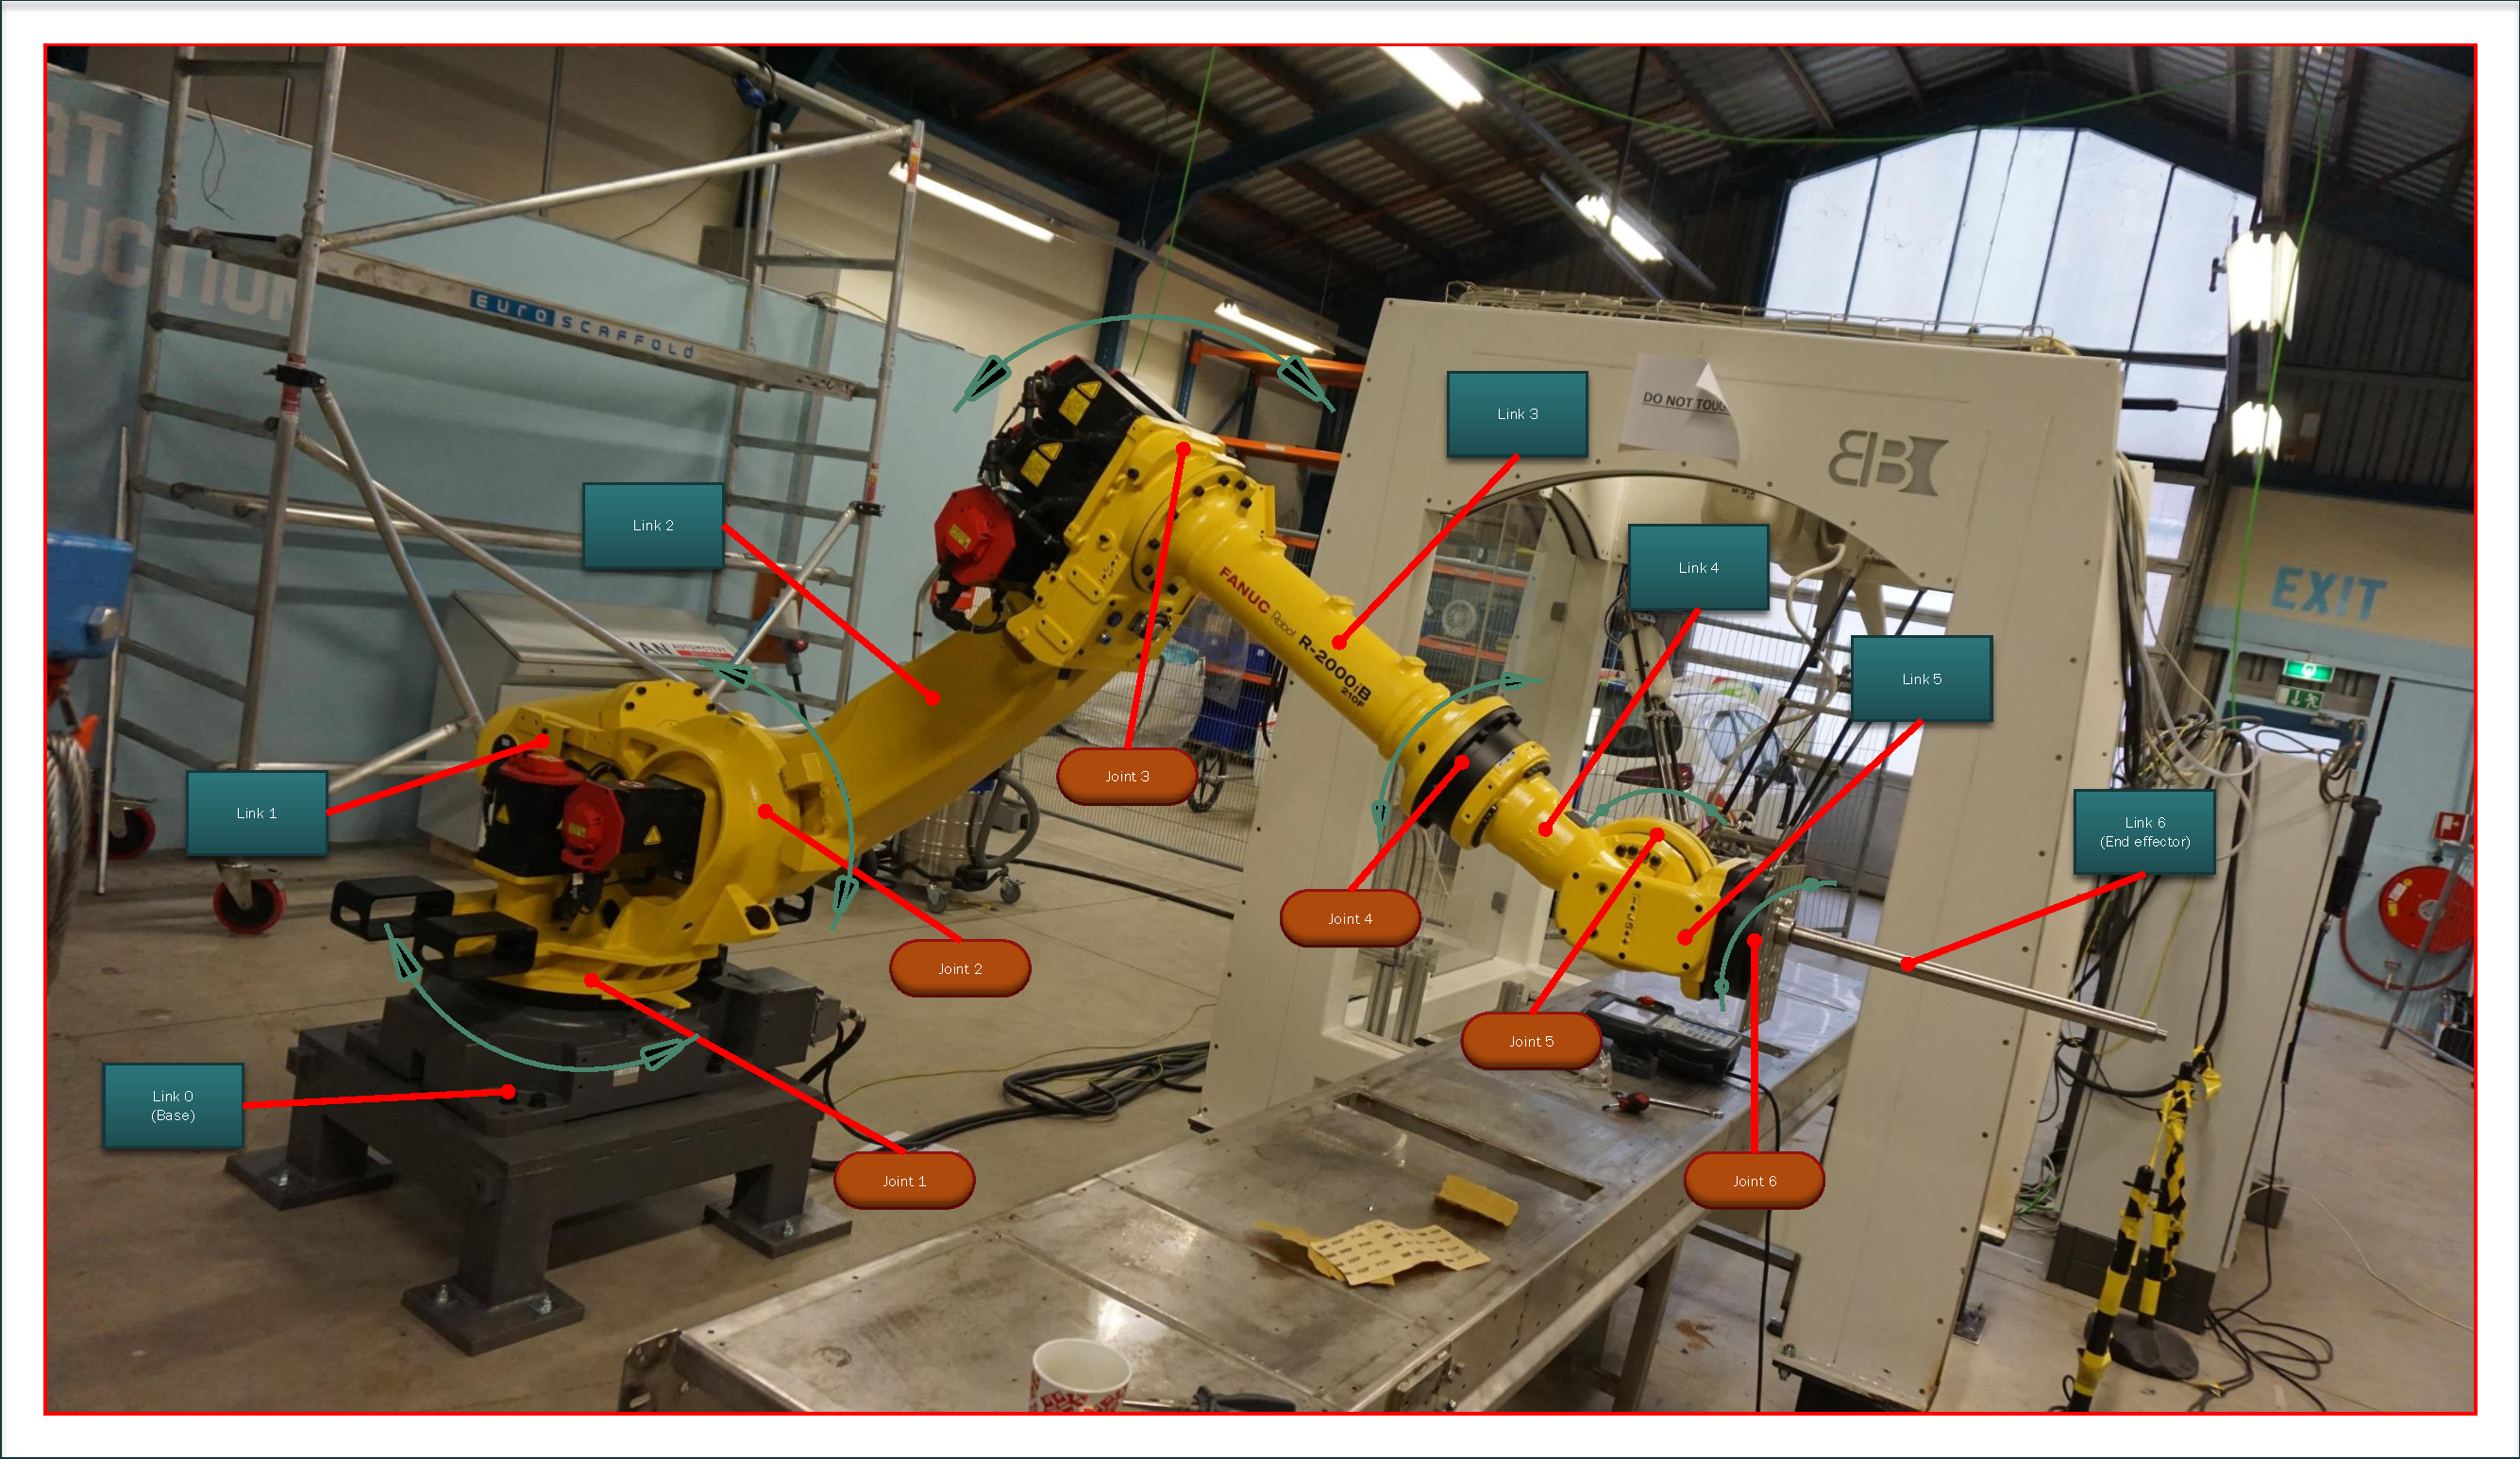
\includegraphics[
	width=1\linewidth,
	center,
	keepaspectratio,
	]{linksANDjoints/linksAndJoints}
	\caption{Links (turquoise) and joints (orange) in the FANUC 210F}
	\label{fig:LinksANDJoints210F}
\end{figure}



\section{local coordinate reference frames}
With the Denavit-Hartenberg convention, local coordinate frames can be attached to the far end of the links $ (i) $ and their accompanying joints $ (i+1) $.
Each link $(i)$ is described relative to the pose of the preceding link.

%\paragraph{Assignation of coordinate frames}


\paragraph{Assignation of $z_i$ axes}

With the DH-notation, the $z_i$ axes are assigned to link $(i)$.
Two cases need to be considered: %regarding joint $(i+1)$:
\begin{itemize}[wide=\parindent]
	\item[\textbf{revolute:}] $z_i$ is the axis of revolution of joint $(i+1)$
	\item[\textbf{prismatic:}] $z_i$ is the axis of translation of joint $(i+1)$
\end{itemize}
%of joint $(i+1)$
This means, that joint $z_i$ turns around axis $z_i$.

\paragraph{Direction of rotation}
With the direction of the $z_i$-axis, the direction of positive rotation around joint $(i+1)$ is also given by the right hand rule (see \cite{Angela_U1S2P1} at 10:35). This means, the direction of positive rotation is counter-clockwise around the $z_i$-axis.

\paragraph{$z_i$ axes in Fanuc 210F}
As described above, the $z_i$ axes can be attached to the Fanuc 210F (see figure \ref{fig:zi_Axes}).

\begin{figure}[H]
	\includegraphics[
	width=1\linewidth,
	center,
	keepaspectratio,
	]{coordinateFrames/z_axes}
	\caption{$z_i$ axes on the Fanuc 210F with the direction of positive rotation (orange)}
	\label{fig:zi_Axes}
\end{figure}

\paragraph{Base frame}

The base frame $(0)$ can be chosen nearly arbitrarily. The origin of the base frame can be any point on $z_0$. For simplicity, the origin of frame$(0)$ can be put into joint$(1)$.  Usually, the x-axis of the base frame is chosen, so that it points in the direction of the \ac{EOAT} in default position according to its base, \cite{DenavitHartenbergKonventionen} but can be chosen in any convenient manner \cite{SpongDynContr}.

\paragraph{Assignation of frames $(i)$}

Starting from frame $(0)$ in an iterative process, frame $(i)$ can be set up using frame $(i-1)$.

Three cases regarding the relationship of axes $z_{i-1}$ and $z_i$  need to be considered when setting up frames:
\begin{itemize}[wide=\parindent] %option solves alignment problem for item label %https://tex.stackexchange.com/questions/246394/alignment-of-labels-in-itemize-with-text-of-document 
	\item[\textbf{Non coplanar:}] Axes don't intersect and are not parallel. Line containing the common normal $z_{i-1}$ to $z_i$ defines $x_i$-axis and the point of intersection with $z_i$ is the origin of frame $(i)$
	\begin{enumerate}[label=\emph{\alph*)}]
		\item find common normal of the joint axes
		\item put origin in intersection of normal with joint axis
		\item put $z_i$ axis in the joint axis
		\item $x_i$ points in direction of the common normal, facing away from frame $(0)$
		\item add $y_i$ according to right hand rule
	\end{enumerate}
	\item[\textbf{Parallel:}] Axes are parallel. Line containing the normal through origin of frame $(i+1)$ and the $z_i$-axis defines the $x_i$-axis which is directed from origin of frame $(i)$ toward the distal joint. The point of intersection of common normal with $z_i$-axis gives the origin of frame $(i)$. % found a mistake here with common normal in \cite{ConstantinForwardKA} witht he help of \cite{SpongDynContr}. The x-axis should point towards next joint, but he says, should point towards last joint, but does it actually the other way around.
		\begin{enumerate}[label=\emph{\alph*)}]
		\item look for normal originating from distal joint
		\item put origin in the intersection of the normal with the joint axis
		\item put the $z_i$ axis in the joint axis of the link $(i+1)$ 
		\item $x_i$ points follows the common normal with the distal joint, pointing towards the distal joint
		\item add $y_i$ according to right hand rule
	\end{enumerate}
	\item[\textbf{Intersecting:}] Axes are intersecting. Line containing the normal to the plane formed by axes $z_{i-1}$ and  $z_i$ gives the $x_i$-axis with positive direction chosen arbitrarily. Point of intersection of  axes $z_{i-1}$  and  $z_i$ is the origin of frame $(i)$.
		\begin{enumerate}[label=\emph{\alph*)}]
		\item put origin in intersection point of the axes
		\item put the $z_i$ axis in the joint axis of the link $(i+1)$
		\item $x_i$ is perpendicular to both joint axes
		\item add $y_i$ according to right hand rule
	\end{enumerate}
\end{itemize}

\paragraph{Assignation of \ac{EOAT} frame}
As there is no distal joint for the \ac{EOAT} frame, the steps for this frame are different:

\begin{enumerate}[label=\emph{\alph*)}]
	\item put origin on axis of proximal joint 
	\item axis $z_i$ follows direction of $z_{i-1}$
	\item $x_i$ can be chosen arbitrarily, but is usually determined by screw holes
	\item add $y_i$ according to right hand rule
\end{enumerate}

\paragraph{local coordinate reference frames on the Fanuc 210F}

As described above, the local coordinate reference frames can also be attached to the Fanuc 210F as seen in \ref{fig:RefFrame}. 

\begin{figure}[H]
	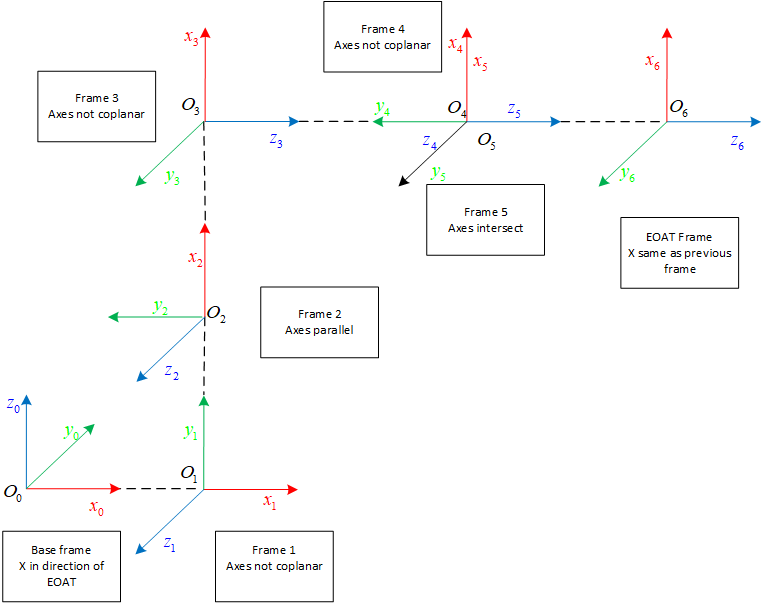
\includegraphics[
	width=1\linewidth,
	center,
	keepaspectratio,
	]{coordinateFrames/CoordinateFrames}
	\caption{Coordinate reference frames for Fanuc 210F}
	\label{fig:RefFrame}
\end{figure}

\paragraph{frame 0 (Base)}
The frame mapping starts with the base frame. For the base frame the z-axis is given through joint $j_1$. Origin of frame 0 is put into joint 1.
The x-axis is chosen to point in direction of of the \ac{EOAT} in standard pose. For standard pose see \ref{fig:StandardPose}.
This pose will also be chosen for alignment of all distal frames.
\begin{figure}[h]
	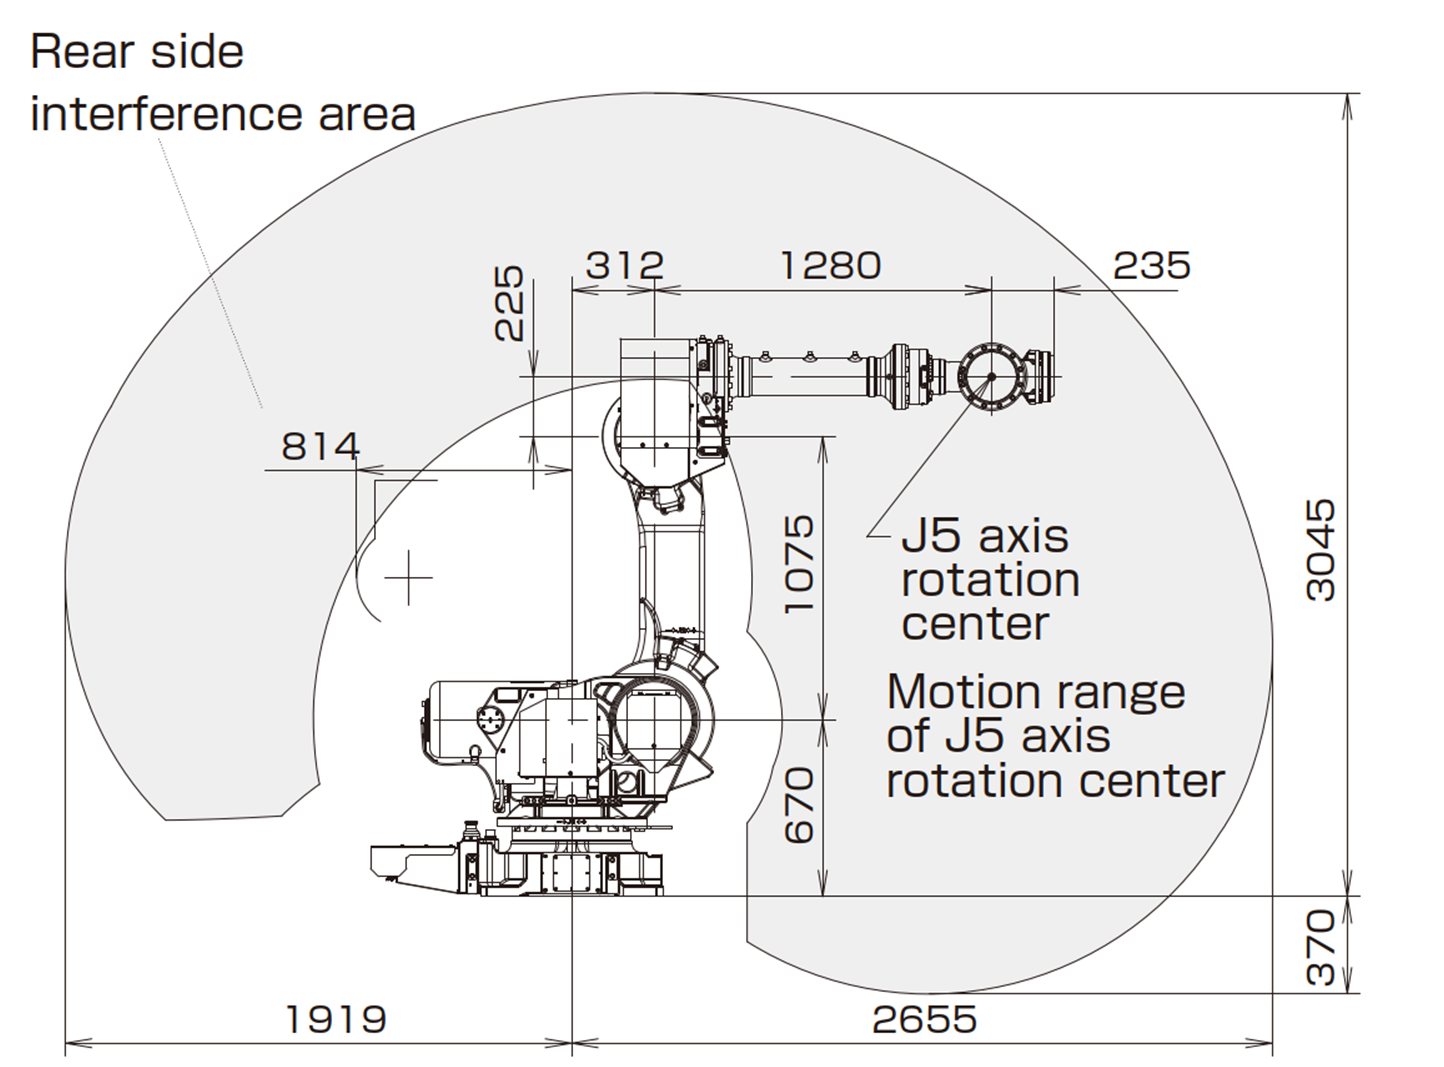
\includegraphics[
	width=1\linewidth,
	center,
	keepaspectratio,
	]{coordinateFrames/standardPose}
	\caption{Standard pose of the robot}
	\label{fig:StandardPose}
\end{figure}

\paragraph{frame 1}
For frame 1, the z-axes are not coplanar. 
Because of that, the  $z_0$-axis is extended until a common normal can be found that intersects with $z_i$ to define the origin $O_1$.
$x_1$ departs from $O_1$ along the common normal.
$y_1$ is added according to the right hand rule.

\paragraph{frame 2}
As seen, in image \ref{fig:zi_Axes}, axes $z_2$ and $z_1$ are parallel. $O_2$ can be found at the intersection of the normal through $O_1$ with $z_2$. $x_2$ follows the common normal with joint 4.
$y_2$ is added according to the right hand rule.

\paragraph{frame 3}
Joint 3 and joint 4 are not exactly aligned (see image \ref{fig:StandardPose}), which prevents the z-axes to intersect. That's why axes $z_3$ and $z_2$ are not coplanar. 
$z_3$ runs parallel through the link 3, due to the orientation of the rotational axis.
As the common normal between $z_3$ and $z_2$ defines $x_3$, which in turn gives $O_3$, the origin can be found far away from the physical position of the joint.
$y_3$ is added according to the right hand rule.

\paragraph{frame 4}
Joint 5 lies in line with joint 4.
As $z_3$ follows this line, the axes  $z_4$ and $z_3$ intersect in the center of joint 5, which gives $O_4$. 
$x_4$ leaves the plane spanned by  $z_4$ and $z_3$ perpendicular.
The positive direction of $x_4$ is chosen to be similar as in frame 3 for simplicity.
$y_4$ is added according to the right hand rule and points in direction of frame 3.

\paragraph{frame 5}
As $z_5$ lies  in line with $O_4$, the axes  $z_5$ and $z_4$ intersect in $O_4$ which puts $O_5$ at the same position as $O_4$.
$x_5$ leaves the plane spanned by  $z_5$ and $z_4$ perpendicular.
The positive direction of $x_5$ is chosen to be similar as in frame 4 for simplicity, which puts $x_5$ and $x_4$ on top of each other. 
$y_5$ is added according to the right hand rule and as $z_5$ is turned 90 degrees relative to $z_4$ around $x_{4,5}$, $y_5$ is turned 90 degrees relative to $z_4$ around $x_{4,5}$ as well.

\paragraph{frame 6 (EOAT)}
$z_6$ lies in line with $z_5$ and is consequently parallel.
as there are no distal joints, to reference $x_6$, it can be chosen arbitrarily. 
For simplicity, it is chosen to be similar as in frame 5. 
$y_6$ is added according to the right hand rule.






